\documentclass[a4paper,10pt]{report}
\usepackage[latin1]{inputenc}
\usepackage{amsmath}
\usepackage{amsmath,bm}
\usepackage{amsthm}
\usepackage{mathtools}
\usepackage{amsfonts}
\usepackage{amssymb}
\usepackage{verbatim}
\usepackage{graphicx}
\usepackage{array}
\usepackage{booktabs}
\usepackage{hyperref}
\usepackage{multicol}
\usepackage{makecell}
\usepackage[margin=0.5in]{geometry}
\usepackage[framemethod=tikz]{mdframed}
\newcommand{\myvec}[1]{\ensuremath{\begin{pmatrix}#1\end{pmatrix}}}
\let\vec\mathbf
\newcommand{\mydet}[1]{\ensuremath{\begin{vmatrix}#1\end{vmatrix}}}
\providecommand{\mbf}{\mathbf}
\providecommand{\pr}[1]{\ensuremath{\Pr\left(#1\right)}}
\providecommand{\qfunc}[1]{\ensuremath{Q\left(#1\right)}}
\providecommand{\sbrak}[1]{\ensuremath{{}\left[#1\right]}}
\providecommand{\lsbrak}[1]{\ensuremath{{}\left[#1\right.}}
\providecommand{\rsbrak}[1]{\ensuremath{{}\left.#1\right]}}
\providecommand{\brak}[1]{\ensuremath{\left(#1\right)}}
\providecommand{\lbrak}[1]{\ensuremath{\left(#1\right.}}
\providecommand{\rbrak}[1]{\ensuremath{\left.#1\right)}}
\providecommand{\cbrak}[1]{\ensuremath{\left\{#1\right\}}}
\providecommand{\lcbrak}[1]{\ensuremath{\left\{#1\right.}}
\providecommand{\rcbrak}[1]{\ensuremath{\left.#1\right\}}}
\begin{document}
\raggedleft FWC22037\vspace{2mm}\\
\centering\Large\textbf{ASSIGNMENT-OPTIMIZATION}\vspace{5mm}
\begin{multicols}{2}
\centering \large\textsc{C}\footnotesize\textsc{ONTENTS}\vspace{5mm}\\
\raggedright\large\textbf{1\hspace{1cm}Problem}\hspace{5.2cm}1\vspace{5mm}\\
\raggedright\large\textbf{2\hspace{1cm}Solution}\hspace{5.25cm}1\vspace{5mm}\\
\raggedright\large\textbf{3\hspace{1cm}Construction}\hspace{4.25cm}2\vspace{5mm}\\
\centering \large\textsc{1  P}\footnotesize\textsc{ROBLEM}\vspace{5mm}\\
	\raggedright\large{Let $f(x)$ is a cubic polynomial which has a local maxima at x=-1.If $f(2) = 18$, f(1)= -1 and $f'(x) = -1$ has local minimum at x=0,then \\
 	(a) The distance between (-1,2) and (a,f(a)) where x=a is a point of local minima is 2$\sqrt{5}$ \\
 	(b) $f(x)$ is increasing for $x \in [1,2\sqrt{5}]$\\
 	(c) $f(x)$ has local minima at x=1\\
 	(d) The value of $f(0)$ is 5 }\\\vspace{5mm}
\centering \large\textsc{2  S}\footnotesize\textsc{OLUTION}\vspace{5mm}\\
\raggedright\large{1.Let the cubic polynomial equation be \begin{align}
 f(x) = ax^3+bx^2+cx+d
 \end{align} } \\
2.Given that  $f(2)=18$
 \begin{align}
 8a+4b+2c+d=18
 \end{align}
3.Given that $f(1) = -1$
 \begin{align}
 a+b+c+d=-1\\
 \frac{df(x)}{dx} = 3ax^2+2bx+c\\
 f'(-1)=0\\
 3a-2b+c =0\\
 \frac{df'(x)}{dx} = 6ax+2b\\
 f''(0) = 0\\
 b=0
 \end{align}
4.Solving Eqs(2)(3)and (6) by substituting b=0 we get
\begin{align}
8a+2c+d=18\\
a+c+d=-1\\
3a+c=0
\end{align}
5.Solving Eqs(10)(11)(12)
\begin{align*}
\myvec {8&2&1&18 \\ 1&1&1&-1 \\ 3&1&0&0} \\ 
R_1 =\frac{R_1}{8}\\
\myvec {1&\frac{1}{4}&\frac{1}{8}&\frac{9}{4} \\ 1&1&1&-1 \\ 3&1&0&0} \\
R_2 = R_2-R_1\\
\myvec {1&\frac{1}{4}&\frac{1}{8}&\frac{9}{4} \\ 0&\frac{3}{4}&\frac{7}{8}&-\frac{13}{4} \\ 3&1&0&0} \\
R_3 = R_3-3R_1\\
\myvec {1&\frac{1}{4}&\frac{1}{8}&\frac{9}{4} \\ 0&\frac{3}{4}&\frac{7}{8}&-\frac{13}{4} \\ 0&\frac{1}{4}&-\frac{3}{8}&-\frac{27}{4}}\\  
R_2 = \frac{4}{3}R_2\\
 \myvec {1&\frac{1}{4}&\frac{1}{8}&\frac{9}{4} \\ 0&1&\frac{7}{6}&-\frac{13}{3} \\ 0&\frac{1}{4}&-\frac{3}{8}&-\frac{27}{4}}\\
 R_1 = R_1 - \frac{R_2}{4}\\
\myvec {1&0&-\frac{1}{6}&\frac{10}{3} \\ 0&1&\frac{7}{6}&-\frac{13}{3} \\ 0&\frac{1}{4}&-\frac{3}{8}&-\frac{27}{4}}\\
R_3 = R_3 - \frac{R_2}{4}\\
\myvec {1&0&-\frac{1}{6}&\frac{10}{3} \\ 0&1&\frac{7}{6}&-\frac{13}{3} \\ 0&0&-\frac{2}{3}&-\frac{17}{3}} \\
R_3 = -\frac{3}{2}R_3\\
 \myvec {1&0&-\frac{1}{6}&\frac{10}{3} \\ 0&1&\frac{7}{6}&-\frac{13}{3} \\ 0&0&1&\frac{17}{2}} \\
 R_1 = R_1 + \frac{R_3}{6}\\
\myvec {1&0&0&\frac{19}{4} \\ 0&1&\frac{7}{6}&-\frac{13}{3} \\ 0&0&1&\frac{17}{2}} \\
R_2 = R_2 - \frac{7}{6}R_3
\myvec {1&0&0&\frac{19}{4} \\ 0&1&0&-\frac{57}{4} \\ 0&0&1&\frac{17}{2}}
\end{align*}
5. From which we can get a = $\frac{19}{4}$, b=0 , c = $\frac{57}{4}$ , d = $\frac{17}{2}$ \\
eq(1) can be modified as \begin{align} 19x^3 -57x+34=0 
\end{align}
For Maxima : \\
    Using gradient ascent method,
    \begin{align}
    x_n=x_{n-1}+\mu\frac{df(x)}{dx}\\
    \frac{df(x)}{dx} = 3ax^2+2bx+c 
    \end{align}
    \raggedright substituting eq 15 in 14 \\
    \raggedright $x_n =x_{n-1}+\mu(3ax^2+2bx+c)$ \\
    \raggedright taking $x_0 = -1, \mu = 0.001 ,precision = 0.00000001$ values obtained using python are :
    \begin{align}
\boxed{\text{Maxima} = 72.0} \\
\boxed{\text{Maxima Point} = -1.0}
\end{align}
For Minima : \\
    Using gradient decent method,
    \begin{align}
    x_n=x_{n-1}-\mu\frac{df(x)}{dx}\\
    \end{align}
    substituting eq 15 in 14 \\
    $x_n=x_{n-1}-\mu(3ax^2+2bx+c)$ \\
    taking $x_0 = -1, \mu = 0.001 ,precision = 0.00000001$ values obtained using python are :
    \begin{align}
\boxed{\text{Maxima} = -4.0} \\
\boxed{\text{Maxima Point} = 1.0}
\end{align}
\centering{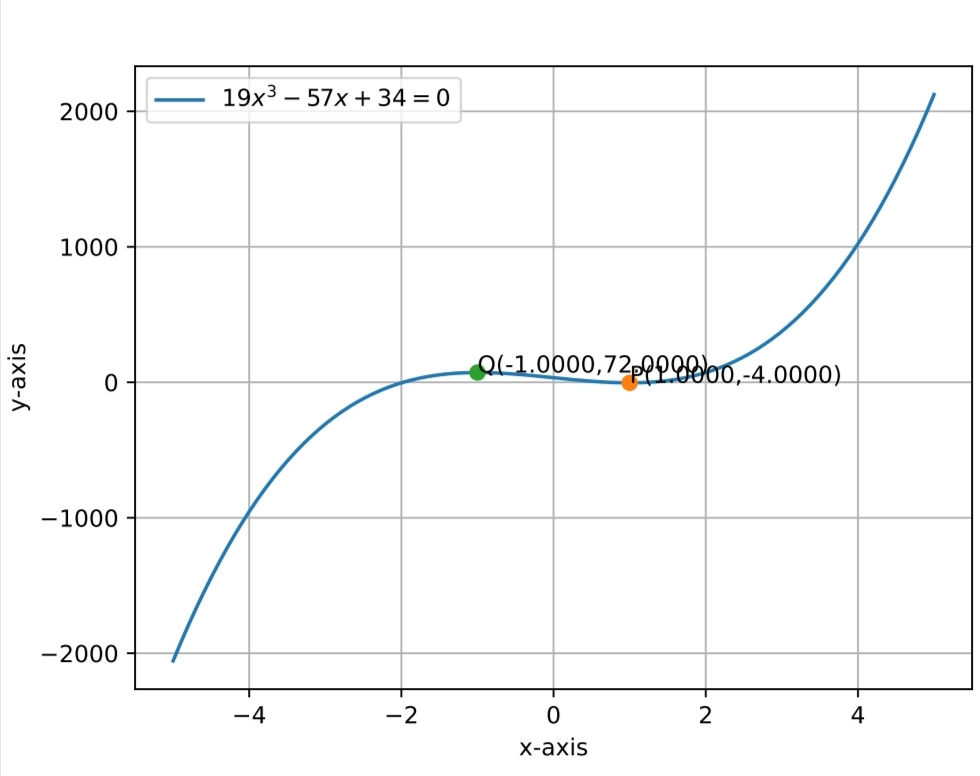
\includegraphics[scale=0.2]{opt-2.jpg}}\vspace{2mm}\\
\raggedright\large{The python code provided in the below source code link.} \\
\begin{mdframed}
\raggedright\large{https://github.com/sivagayathri \\ /FWC/blob/main/opt/opt-2.py}
\end{mdframed}
\end{multicols}
\end{document}
